\chapter{Diagrammes de séquence (seq)}
\section{TITRE A CHANGER 1}
%\begin{figure}[H]
%	\centering
%	\includegraphics[width=1\linewidth]{diagrams/bathroom/}
%	\caption{TODO}
%	\label{fig:diagramme_seq1}
%\end{figure}

\section{Diagramme de séquence lors de l'entré d'un utilisateur dans la douche}
Le diagramme ci-dessous présente le déroulement des actions en fonction des différentes capteurs (capteur de charge, capteur de position), du contrôleur et de la dalle élévatrice. 

Les capteurs fournissent des informations (présence ou non du locataire dans la douche, hauteur du locataire) qui analyse l'arrivée de ces flux en continu (\textbf{loop}) puis qui procède au traitement afin d'élever ou d'abaisser la dalle élévatrice. 
\begin{figure}[H]
	\centering
	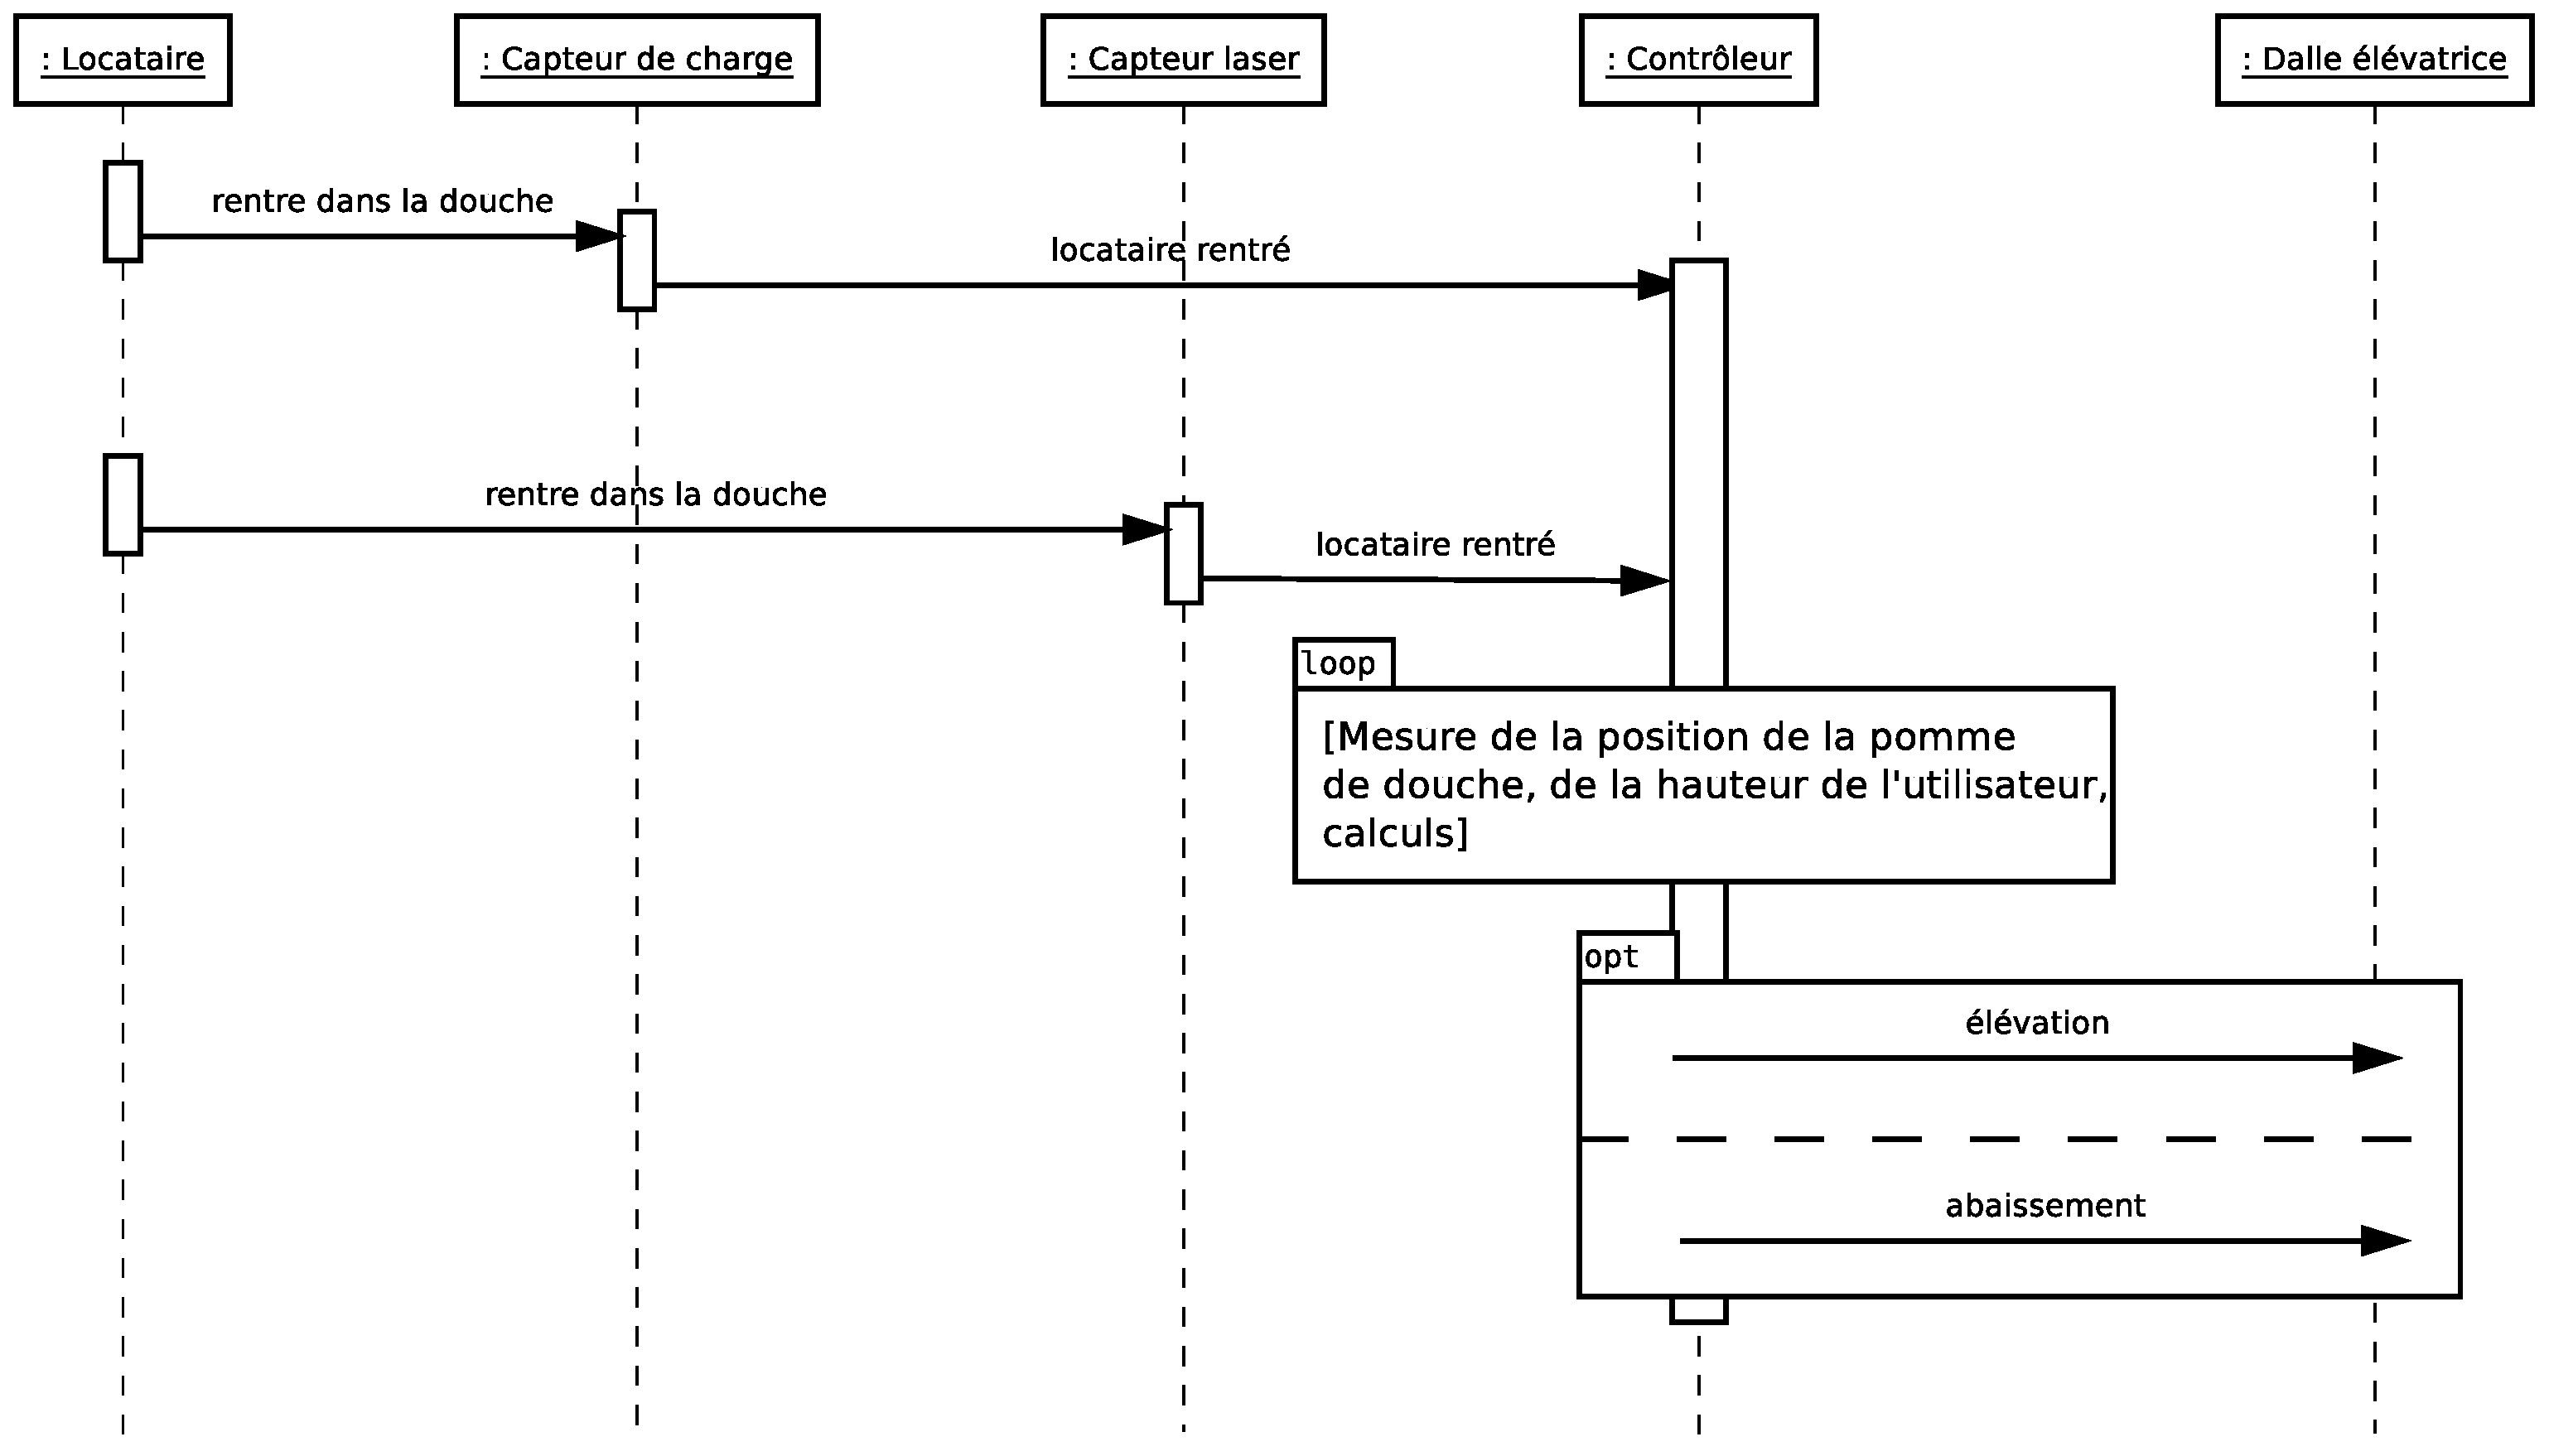
\includegraphics[width=1\linewidth]{diagrams/bathroom/diagramme_sequence2.eps}
	\caption{Diagramme de séquence lors de l'entré d'un utilisateur dans la douche}
	\label{fig:diagramme_seq2}
\end{figure}
